\documentclass[11pt,letterpaper]{article}
\usepackage[top=3cm, bottom=2cm, left=2cm, right=2cm, columnsep=20pt]{geometry}
\usepackage{pdfpages}
\usepackage{graphicx}
\usepackage{etoolbox}
\apptocmd{\sloppy}{\hbadness 10000\relax}{}{}
% \usepackage[numbers]{natbib}
\usepackage[T1]{fontenc}
\usepackage{ragged2e}
\usepackage[french]{babel}
\usepackage{listings}
\usepackage{color}
\usepackage{soul}
\usepackage[utf8]{inputenc}
\usepackage[export]{adjustbox}
\usepackage{caption}
\usepackage{amsmath}
\usepackage{amssymb}
\usepackage{float}
\usepackage{csquotes}
\usepackage{fancyhdr}
\usepackage{wallpaper}
\usepackage{siunitx}
\usepackage[indent]{parskip}
\usepackage{textcomp}
\usepackage{gensymb}
\usepackage{multirow}
\usepackage[hidelinks]{hyperref}
\usepackage{abstract}
\renewcommand{\abstractnamefont}{\normalfont\bfseries}
\renewcommand{\abstracttextfont}{\normalfont\itshape}
\usepackage{titlesec}
\titleformat{\section}{\large\bfseries}{\thesection}{1em}{}
\titleformat{\subsection}{\normalsize\bfseries}{\thesubsection}{1em}{}
\titleformat{\subsubsection}{\normalsize\bfseries}{\thesubsubsection}{1em}{}

\usepackage{xcolor}
\definecolor{codegreen}{rgb}{0,0.6,0}
\definecolor{codegray}{rgb}{0.5,0.5,0.5}
\definecolor{codepurple}{rgb}{0.58,0,0.82}
\definecolor{backcolour}{rgb}{0.95,0.95,0.92}
\lstdefinestyle{mystyle}{
    backgroundcolor=\color{backcolour},   
    commentstyle=\color{codegreen},
    keywordstyle=\color{magenta},
    numberstyle=\tiny\color{codegray},
    stringstyle=\color{codepurple},
    basicstyle=\ttfamily\footnotesize,
    breakatwhitespace=false,         
    breaklines=true,                 
    captionpos=b,                    
    keepspaces=true,                 
    numbers=left,                    
    numbersep=5pt,                  
    showspaces=false,                
    showstringspaces=false,
    showtabs=false,                  
    tabsize=2
}
\lstset{style=mystyle}

\usepackage[most]{tcolorbox}
\newtcolorbox{note}[1][]{
  enhanced jigsaw,
  borderline west={2pt}{0pt}{black},
  sharp corners,
  boxrule=0pt, 
  fonttitle={\large\bfseries},
  coltitle={black},
  title={Note:\ },
  attach title to upper,
  #1
}

%----------------------------------------------------

\setlength{\parindent}{0pt}
\DeclareCaptionLabelFormat{mycaptionlabel}{#1 #2}
\captionsetup[figure]{labelsep=colon}
\captionsetup{labelformat=mycaptionlabel}
\captionsetup[figure]{name={Figure }}
\newcommand{\inlinecode}{\normalfont\texttt}
\usepackage{enumitem}
\setlist[itemize]{label=\textbullet}

\begin{document}
\begin{titlepage}
\center

\begin{figure}
    \ThisULCornerWallPaper{.4}{Polytechnique_signature-RGB-gauche_FR.png}
\end{figure}
\vspace*{2 cm}

\textsc{\Large \textbf{PHS2223 --} Introduction à l'optique moderne}\\[0.5cm]
\large{\textbf{Équipe : 04}}\\[1.5cm]

\rule{\linewidth}{0.5mm} \\[0.5cm]
\Large{\textbf{Expérience 3}} \\[0.2cm]
\text{Mesure de polarisation}\\
\rule{\linewidth}{0.2mm} \\[2.3cm]

\large{\textbf{Présenté à}\\
  Guillaume Sheehy\\
  Esmat Zamani\\[2.5cm]
  \textbf{Par :}\\
  Émile \textbf{Guertin-Picard} (2208363)\\
  Laura-Li \textbf{Gilbert} (2204234)\\
  Tom \textbf{Dessauvages} (2133573)\\[3cm]}

\large{\today\\
Département de Génie Physique\\
Polytechnique Montréal\\}

\end{titlepage}

%----------------------------------------------------

\tableofcontents
\pagenumbering{roman}
\newpage

\pagestyle{fancy}
\setlength{\headheight}{14pt}
\renewcommand{\headrulewidth}{0pt}
\fancyfoot[R]{\thepage}

\pagestyle{fancy}
\fancyhf{}
\renewcommand{\headrulewidth}{1pt}
\fancyhead[L]{\textbf{PHS2223}}
\fancyhead[C]{Rapport préliminaire}
\fancyhead[R]{\today}
\fancyfoot[R]{\thepage}

\pagenumbering{arabic}
\setcounter{page}{1}

%----------------------------------------------------

\section{Introduction}

Les ondes électromagnétiques ont plusieurs propriétés qui permettent d'expliquer les différents
phénomènes optiques observés dans la vie de tous les jours. L'une d'entre elles est la polarisation,
qui dicte la direction d'oscillation du champ électrique dans une onde électromagnétique. Elle
est fréquemment utilisée pour faire fonctionner différents objets communs, tels que des écrans à
cristaux liquides et des verres polarisés pour des lunettes. Ce laboratoire se concentre sur l'analyse
de cette propriété dans un système optique. Pour se faire, une expérience de mesure de puissance sera
faite avec des filtres polariseurs linéaires, qui permettent de ne laisser passer qu'une seule polarisation de
la lumière. Différents nombres et différentes orientations des polariseurs seront testés en laboratoire, mais
aussi modélisés mathématiquement au préalable. Ces modélisations seront faites à l'aide de deux formalismes, soit
le classique où l'expression standard d'une onde électromagnétique classique est utilisée, et le formalisme de
Jones, où l'état de polarisation d'une onde est décrit par un vecteur d'état (ou de Jones). Le document présent détaille
le fondement théorique de la polarisation et de ses formalismes, détaille les montages qui seront utilisés
pour l'expérience, et émet des hypothèses sur les observations à faire en laboratoire à l'aide du modèle
mathématique.

\section{Théorie}\label{theo}
Cette section présente les principes physiques et les méthodes mathématiques importantes à l'expérience à réaliser.

\subsection{Polarisation}
La polarisation est une propriété physique de la lumière, et des ondes électromagnétiques, correspondant à une mesure de l'orientation du champ électromagnétique. En d'autres termes, ce principe permet de déterminer la direction des oscillations, plus précisément celle d'un champ électrique \textcolor{red}{(Source 1)}. Plusieurs types de polarisation peuvent être observés tels que la polarisation linéaire, circulaire, et elliptique. Dans le cas linéaire, les ondes n'ont aucune différence de phases entre le champ électrique en $x$ et celui en $y$. Cette polarisation linéaire peut être écrite par l'équation suivante \textcolor{red}{(Source 2)} :
\begin{equation}
  \vec{E}_{0}=(E_{x},E_{y},0)
  \label{pol_lin}
\end{equation}
La direction de la polarisation normalisée, dans le cas ci-dessus, peut alors être déterminée à l'aide de l'équation suivante :
\begin{equation}
  \hat{P}=\frac{E_{x}\hat{x}+E_{y}\hat{y}}{\sqrt{E_{x}^{2}+E_{y}^{2}}}
\end{equation}
La polarisation elliptique résulte d'une combinaison linéaire de composantes ayant une différence de phase et un rapport d'amplitude de valeurs arbitraires. Pour la polarisation circulaire, celle-ci correspond à une polarisation elliptique ayant une différence de phase de 90$^\circ$, pouvant alors être écrite de la manière suivante \textcolor{red}{(Source 3)} :
\begin{equation}
  \vec{E}_{0}=(E_{0},E_{0}e^{i\frac{\pi}{2}},0)
\end{equation}
Ainsi, lors d'une polarisation linéaire, le champ électrique est confiné sur un plan unique dans la direction de propagation, alors que, dans le cas des deux autres polarisations, le champ électrique rotationne à mesure que l'onde se propage.

% Source 1 : https://science.nasa.gov/ems/02_anatomy/
% Source 2 : Harvard pdf
% Source 3 : https://www.idex-hs.com/resources/resources-detail/understanding-polarization

\subsubsection{Polariseurs}
Afin d'obtenir une certaine polarisation, les polariseurs, dispositifs permettant de filtrer la lumière, sont utilisés. Le fonctionnement de ces polariseurs consiste à sélectionner certaines ondes spécifiques de sorte que celles-ci aient une direction particulière \textcolor{red}{(Source 4)}. Ces polariseurs peuvent être divisés en trois catégories : réfléchissants, dichroïques, et biréfringents. Les polariseurs réfléchissants ont pour principe de transmettre les ondes souhaitées, tout en réfléchissant celles non-désirées. Dans le cas des dichroïques, ceux-ci, au lieu de réfléchir les faisceaux non-désirés, absorbent une polarisation spécifique et transmettent les autres. Finalement, les polariseurs biréfringents utilisent un cristal anisotrope pour séparer un faisceau lumineux en composantes de polarisation, ainsi ce type de polariseurs utilisent la dépendance de la polarisation à l'indice de réfraction \textcolor{red}{(Source 5)}.

% Source 4 : Modern electrodynimics, Zangwill Chapter 16.

% Source 5 : https://www.edmundoptics.fr/knowledge-center/application-notes/optics/introduction-to-polarization/

\subsection{Modèle classique}
Les ondes électromagnétiques, telles que la lumière, correspondent à des perturbations oscillantes des champs électriques et magnétiques. Ces champs, perpendiculaires l'un à l'autre, oscillent également perpendiculairement à la direction de propagation de l'onde, formant une configuration tridimensionnelle caractéristique des ondes transervales. Ces ondes, comparativement aux ondes mécaniques, se propagent à la vitesse de la lumière. Celles-ci, produites par des particules chargées électroniquement en accélération, ne nécessitent aucun milieu de propagation, pouvant alors se propager dans le vide \textcolor{red}{(Source A)}.

Les ondes électromagnétiques sont régies par les équations de Maxwell et, à partir de celles-ci, il est possible d'obtenir les solutions générales aux équations d'onde, soient les ondes planes. Celles-ci, caractérisées par une direction de propagation $r$, une fréquence angulaire $\omega$, et un vecteur d'onde $k$, peuvent être écrites de la forme suivante \textcolor{red}{(Source B)} :
\begin{equation}
  \begin{aligned}
  \mathbf{\Bar{E}}(\textbf{r},t)&=\mathbf{\Bar{E}_{0}}e^{i(\mathbf{kr}-\omega t)} & \;\;\;\;\;\;\;\; & \mathbf{\Bar{H}}(\mathbf{r},t)&=\mathbf{\Bar{H}_{0}}e^{i(\mathbf{kr}-\omega t)} \\
  \end{aligned}
  \label{champs}
\end{equation}
Ensemble, ces deux ondes planes sont des composantes potentielles d'une onde électromagnétique. Cependant, tel que mentionné dans la section précédente, la polarisation concerne la direction du champ électrique, ainsi seulement la première équation $\mathbf{\Bar{E}}$ est considérée. Donc, par exemple, un champ électrique se dirigeant dans la direction $z$ aurait pour équation la suivante :
\begin{equation}
  \vec{E}(z,t)=
  \begin{pmatrix}
    E_{x} \\
    E_{y} \\
    0 \\
  \end{pmatrix}
  e^{i2\pi(\frac{z}{\lambda}-\frac{t}{T})}=
  \begin{pmatrix}
    E_{x} \\
    E_{y} \\
    0 \\
  \end{pmatrix}
  e^{i(kr-\omega t)}
\end{equation}
Où $\lambda$ correspond à la longueur d'onde, et $T$ à la période. Ainsi, en observant l'équation (\ref{pol_lin}), celle-ci représente une polarisation linéaire en $z$.

% Source A : Electromagnetic waves pdf
% Source B : Modern electrodynimics, Zangwill Chapter 16.

\subsubsection{Puissance optique}
La puissance optique correspond à la capacité d'un système optique à converger, ou à diverger, la lumière. Cette puissance peut être calculée à l'aide de la moyenne temporelle du vecteur de Poynting ($\vec{S}$), qui représente la densité de flux lié à la propagation de l'onde.
\begin{equation}
  P=\langle S\rangle=\frac{1}{\eta}|E|^{2}
\end{equation}
Où $\eta$ correspond à l'impédance du milieu de transmission, et $E$ au champ électrique.

\subsection{Modèle de Jones}
En optique, la polarisation de la lumière peut être représentée à l'aide du formalisme de Jones. Cette méthode consiste à décrire les composantes d'un champ, soient les états de polarisation, par un vecteur (2$\times$1), nommé vecteur de Jones $\vec{\mathcal{J}}$, et les composantes polarisantes, soient les éléments optiques, par une matrice (2$\times$2), nommée matrice de Jones $M_{\mathcal{J}}$. De manière spécifique, le vecteur de Jones représente l'amplitude et la phase d'un champ électrique dans les directions $x$ et $y$, ainsi, en utilisant la formulation précédente à l'équation (\ref{champs}) et en ajoutant une phase $\phi$, le vecteur de Jones est donné par :
\begin{equation}
  \vec{\mathcal{J}}=
  \begin{pmatrix}
    E_{0x} \\
    E_{0y}e^{i\Delta\phi} \\
  \end{pmatrix}
\end{equation}
En ce qui concerne la matrice, celle-ci peut subir des rotations, créant ainsi une nouvelle matrice. Cette rotation est décrite par la matrice de rotation suivante.
\begin{equation}
  R(\theta)=
  \begin{pmatrix}
    \cos(\theta) & \sin(\theta) \\
    -\sin(\theta) & \cos(\theta) \\
  \end{pmatrix}
\end{equation}
Où $\theta$ correspond à l'angle de rotation de la matrice. Ne s'appliquant qu'à la lumière entièrement polarisée, ce formalisme est, généralement, utilisé lors du traitement des phénomènes d'interférence et les problèmes de superposition des amplitudes de champ \textcolor{red}{(Source Z)}. À partir de cette formulation, l'état de polarisation résultant $\mathcal{J}$ est, ensuite, déterminée à l'aide d'un produit entre la matrice et le vecteur.
\begin{equation}
  \vec{\mathcal{J}}'=M_{\mathcal{J}}\cdot\vec{\mathcal{J}}
\end{equation}
Le modèle de Jones permet, tout comme le modèle classique, de calculer la puissance optique. Pour ce faire, il est possible d'utiliser le vecteur de Poyinting.
\begin{equation}
  P=\langle S\rangle=\frac{1}{2\eta}\|\vec{\mathcal{J}}\|^{2}
\end{equation}
Où $\eta$ correspond à l'impédance du milieu de transmission, et $\vec{\mathcal{J}}$ est le vecteur de Jones.

% Source Z : https://spie.org/publications/spie-publication-resources/optipedia-free-optics-information/fg05_p57-61_jones_matrix_calculus#_=_

\section{Méthodologie}


\subsection{Présentation des montages}

La méthode utilisée lors de ce laboratoire a pour but de mesurer l'évolution de la puissance transmise par un système optique en fonction de l'angle de polarisation de sa lumière. Les figures \ref{systeme a 2 polarisateur} et \ref{systeme a 3 polarisateur} présente sous la forme d'un schéma les deux circuits étudiés lors de ce laboratoire \textcolor{red}{source enonce}.

\begin{figure}[H]
  \centering
        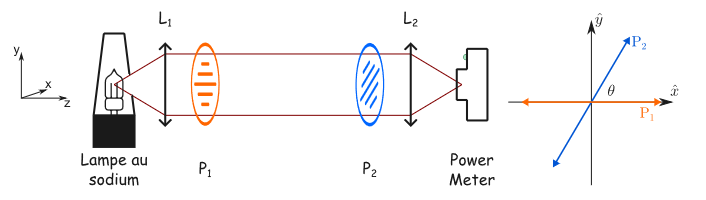
\includegraphics[scale=0.71]{Systeme2polarisateurs.png}
        \caption{Système à 2 polarisateur}
        \label{systeme a 2 polarisateur}
\end{figure}

\begin{figure}[H]
  \centering
        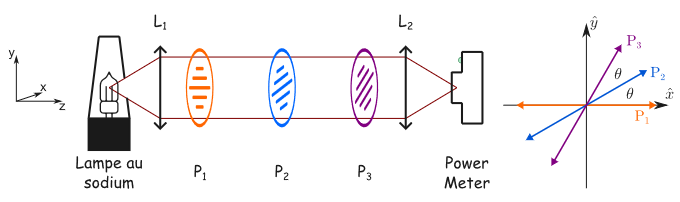
\includegraphics[scale=0.71]{Systeme3polarisateurs.png}
        \caption{Système à 3 polarisateur}
        \label{systeme a 3 polarisateur}
\end{figure}

Chacun des systèmes est constitué d'un lampe au sodium comme source, suivit d'une lentille $L_1$ permettant d'en collimer le faisceaux. Il passera ensuite à travers une série de réseaux de polarisation pour être finalement focalisé par une lentille $L_2$ sur la surface d'un power-meter. Dans les deux systèmes présentés, le réseau de polarisation commence par un polarisateur horizontal $P_1$ suivi d'un polarisateur à angle variable $P_2$ pour le système 2 et de deux polarisateurs à angle variable $P_2$ et $P_3$ pour le système 3.

\subsection{Manipulations}

Pour la système à deux polarisateurs, les séries de mesures à réaliser seront donc :

\begin{enumerate}
    \item Retirez le polariseur $P_2$
    \item Notez la puissance optique transmise par le système comme puissance de référence : $P_0$
    \item Replacez $P_2$ sur l’axe optique et tournez-le afin de maximiser la puissance transmise. Notez cette puissance (P($\theta$ = 0))
\end{enumerate}

Pour le système à trois polarisateurs, les étapes seront donc: 

\begin{enumerate}
    \item Retirez le polariseur $P_2$ et $P_3$
    \item Notez la puissance optique transmise par le système comme puissance de référence : $P_0$
    \item Replacez $P_2$ sur l’axe optique et tournez-le afin de maximiser la puissance transmise.
    \item Replacez $P_3$ sur l’axe optique et tournez-le afin de maximiser la puissance transmise. Notez cette puissance (P($\theta$ = 0))
\end{enumerate}

Dans les deux cas, ces séries de mesures seront réalisées pour des angles compris entre 0° et 115° par incrémentation de 5°. Dans le cas du système à trois polarisateurs, l'angle $\theta$ à mesuré est celui compris entre $P_2$ et $P_3$ tel que présenté à la figure \ref{systeme a 3 polarisateur}.



\section{Hypothèses}

Cette section utilise les deux modèles présentés à la section \ref{theo} pour simuler les mesures de
coefficients de transmission qui pourront être faits avec les montages.

\subsection{Modèle classique}

Avec le modèle classique

les courbes présentées à la figure \ref{classique} montrent la variation
du coefficient de transmission en fonction de la variation de l'angle $\theta$ autant pour le 
système à deux polariseurs qu'à trois polariseurs.

\begin{figure}[H]
  \centering
  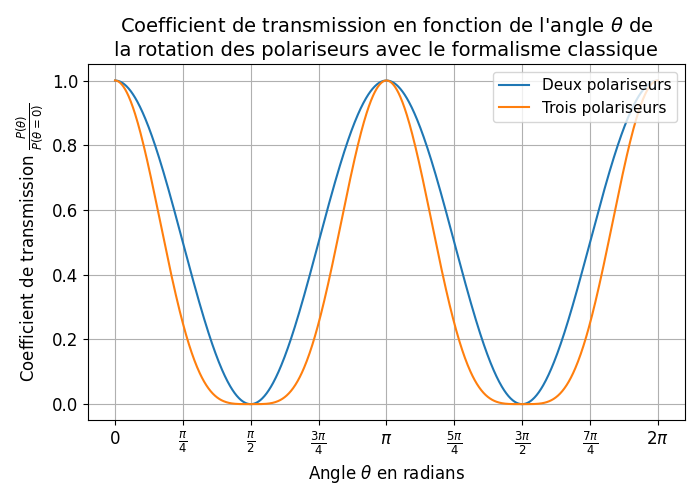
\includegraphics[scale=0.7]{coeff_classique.png}
  \caption{Coefficients de transmission pour le modèle classique.}
  \label{classique}
\end{figure}

Il est donc possible de faire comme hypothèse que le montage à deux polariseurs présente un comportement
sinusoidal entre 0 et 1 pour son coefficient de transmission. Quant au montage à trois polariseurs, cette
courbe est plus aplatie aux minimums et est toujours sous la courbe de deux polariseurs. La puissance est
donc réduite avec l'ajout du polariseur, mais les minimums de puissance restent aux mêmes angles.

\subsection{Modèle de Jones}

La figure \ref{jones} présente les mêmes courbes que pour le modèle classique, mais avec le modèle de Jones.

\begin{figure}[H]
  \centering
  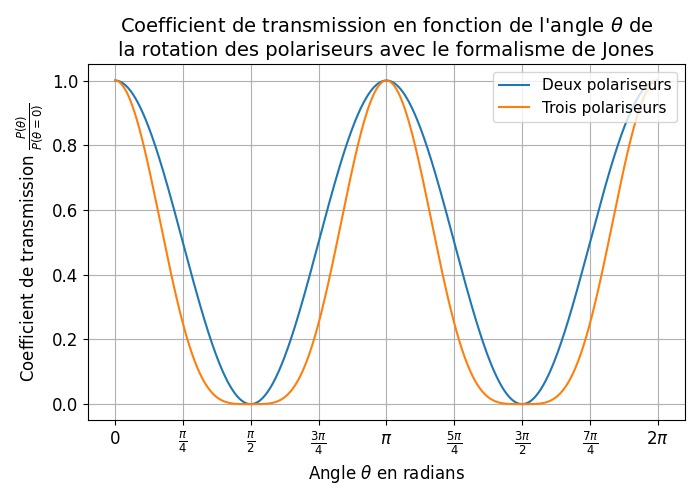
\includegraphics[scale=0.7]{coeff_jones.png}
  \caption{Coefficients de transmission pour le modèle de Jones.}
  \label{jones}
\end{figure}

Il est possible de voir que les résultats sont les mêmes que pour le modèle classique. Les hypothèses à émettre
sont donc les mêmes.


\clearpage

%\bibliographystyle{unsrtnat}
%\bibliography{camera_prelab.bib}

\end{document}
